\section[Dirac-Funktion (Delta-Funktion)]{Dirac-Funktion (Delta-Funktion) $\bm{\delta = \delta(t)}$}

Die Systemantwort eines LTI-Systems auf eine beliebige Anregung $x = x(t)$ kann bestimmt werden, wenn man die Systemantwort auf die 
Dirac-Funktion kennt (Impulsantwort $y_{\delta} = y_{\delta}(t)$) 


\subsection{Darstellung der Dirac-Funktion}

\begin{center}
    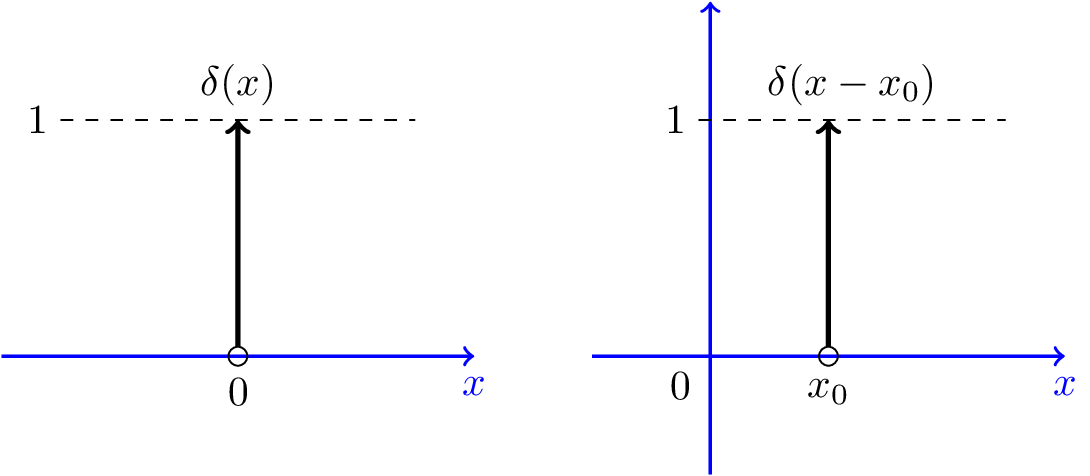
\includegraphics[width=0.7\columnwidth]{images/delta-funktion.png}
\end{center}


\example{Linearkombination mehrerer Dirac-Funktionen}

\vspace{-0.2cm}
$$ 2 \delta(t+1) - \delta(t-2) \qquad \text{ (\textrightarrow\ Ausblendeigenschaft) } $$


\subsection{Eigenschaften der Dirac-Funktion}

\begin{itemize}
    \item Flächeninhalt immer gleich 1 \qquad $\int \limits_{- \infty}^{\infty} \delta(t) \, \diff t = 1$
    \item Unendlich kurzer Impuls \quad $ \delta(t) = 0$ für $t \neq 0$
    \item Für $t = 0$ ist \textbf{kein} Funktionswert definiert; $\neq \infty$
    \item Ausblendeigenschaft (Funktionswerte herausfiltern) \\
        Funktion $f = f(t)$ stetig bei $t = t_0 \in \mathbb{R}$ \qquad  $\int \limits_{- \infty}^{\infty} \delta(t - t_0) \cdot f(t) \, \diff t = f(t_0) $
    \item Dirac-Funktion ist \textbf{verallgemeinerte Ableitung} der (Einheits-) Sprungfunktion \\
        \textrightarrow\ $\delta(t) = \dot{\sigma}(t)$ 
\end{itemize}

